% (c) 2020 Stefan Antonowicz
% Based off of tex found at https://github.com/ludus-leonis/nipajin
% This file is released under Creative Commons
% Attribution-NonCommercial-ShareAlike 4.0 International License.
% Please do not apply other licenses one-way.

\renewcommand{\yggMystics}{%
  \mychapter{Mystics}{mystics}
}

\renewcommand{\yggMysticsText}{%

\flavor{ 
  And it has been said of old that all things that have been were wrought by the small gods, excepting only \TheAuthority, the Authority, the God of Having Done, who made the gods, and hath thereafter rested.  And none may pray to \TheAuthority but only to the gods whom he hath made.
}


\mysection{The Gift of Grace}{mystics-grace}

The Holy Word echoes and reverberates along the branches of Ygg.  The act of trying to understand the Word bestows the Authority's Grace on you.  Grace allows you to perform the \mylink{Seven Sacraments}{mystics-seven-sacraments}, found in the section on \mylink{Arcana}{arcana}

Grace Dice are \POOL, meaning if you roll a Failure (a 1 or a 2) you lose the die until you rest.  You can restore 1 Grace \POOL whenever you Bivouac. You can never use Grace to perform something that requires Faith. 

\mysection{The Crux of Mojo}{mystics-mojo}

\flavor{
    Where's the game in life, behind the game behind the game... \Tilde Public Enemy
}

  While most Mortal connections to magic are driven by control and sacrifice, it is possible to wield magic by yielding to it.  Mojo allows you to tap into the wellspring of magic to protect yourself, harm your enemies, and command the dead.

  Your Mojo is represented as a \UD. You can use your Mojo \UD to power your Aura (see the description of this Virtue in the core rules) and to practice \mylink{Necromancy}{arcana-necromancy}. 


  \cbreak

  \mysection{Cunning}{mystics-cunning}

  Cunning is used during a Vacation to perform the \mylink{Marvel of Occultism}{marvels-occultism}, and be used to help Spriggans create \mylink{magic weapons}{magic-sword}.  Cunning is bound the the Wheel.


  \mysubsection{The Wheel}{mystics-the-wheel}

  Your Cunning moves counterclockwise through a Wheel of eight points - it ascends from the Void to Sickle, Quotidian, and Gibbous to Crown, then descends through Gibbous, Quotidian, and Sickle to return to the Void.
  
  During character creation, roll a d8 to see where your Mojo begins:

  \mytable{X X}{}
  {
    1 & Void \\
    2 & Waning Sickle \\
    3 & Waning Quotidian \\
    4 & Waning Gibbous \\
    5 & Waxing Sickle \\
    6 & Waxing Quotidian \\
    7 & Waxing Gibbous \\
    8 & Crown
  }

  Every Session, move your Mojo one step counter-clockwise along the wheel:

  For some powerful Marvels, you may need to move ”[num] Widdershins” before you can attempt the ritual again. A full Widdershins means you must make [num] transit(s) of the Wheel before you can cast the ritual again. 

    \begin{center}
  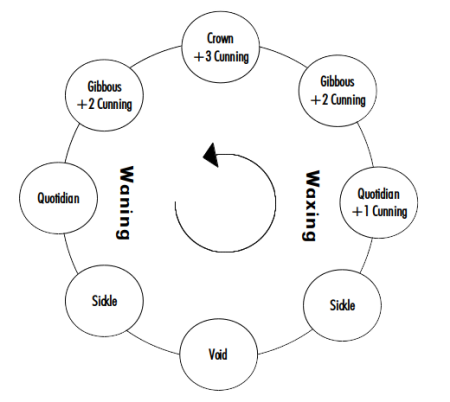
\includegraphics[scale=.3]{mojo_circle}
  \end{center}

  For example, if you were at Crown, you must travel to Waning Gibbous, then Waning Quotidian, etc. all the way back around to Crown before you can try again (meaning you will need to play multiple Sessions). \\~  \\~

  \hrule




  Certain phases of the Wheel (as well as other members of your Coven and your familiar) provide additional Cunning:

  \mytable{X X}{}
  {
    Wheel: Crown & +3 \\
    Wheel: Gibbous & +2 \\
    Wheel: Wax Quotidian & +1 \\
    Coven & +1 each member \\
    Familiar: & +1 if present \\
  }  

  \cbreak

\mysection{The Crux of Faith}{mystics-faith}

It is forbidden to worship \TheAuthority directly; instead, you whisper your prayers and invocations to the Small Gods, the Gods of Doing.  Your Faith (measured as d4 \UD) in your Small God allows you to invoke the Liturgies of the Authority they sit beneath.

Unlike Grace, Faith does not come back when you rest.  You can gain or regain Faith up to your \MAX by actively, aggressively pursing your Small God's influence on Acheron.  You gain Faith \UD completely at the Arbiter's discretion.  Some examples of things that might gain you Faith: slaughtering the priest of a rival cult; converting a crowd of listeners; invoking the name of your Small God and succeeding; eating hallucinogenic mushrooms and tripping balls while your Small God copulates with you, proclaiming your destiny, etc.

It's possible to lose Faith through your actions, as well.  When you do something your Small God doesn't approve of or witnesses something which would shake your belief: a commune of the converted found diseased deformed and starved, a call for help which goes unanswered, a nocturnal visit by a creeping hulking thing which whispers terrible secrets of the endless sky into the your ear heedless to the invocation of your God, you lose Faith Die.

If your Faith Die reach 0, you must immediately roll a d4 - on a Failure (a 1 or a 2) you suffer a \mylink{Crisis of Faith}{table-crisis-of-faith}; otherwise, gain +1 Faith \UD

\newpage

\mysubsection{The Contract}{mystics-the-contract}

The Small Gods must obey certain "rules" when dealing with Mortals:

\mynumlist {
  \item  The Small Gods must be true to their nature
  \item  The Small Gods must hear what Mortals have to say, and they must honor their bargains
  \item  The Small Gods can only hear a Mortal's words - they cannot hear their thoughts
  \item  The Small Gods must speak truth to Mortals about what is happening in distant places
  \item  The Small Gods must prophesy honestly - though they may try to trick Mortals with their words
}

\mysubsection{The Holy Symbol}{mystics-holy-symbol}

Your Holy Symbol allows you to harness your Faith to perform the \mylink{Liturgies}{mystics-liturgies}.  Tell the Arbiter what the Holy Symbol of your Small God is (there are a few ideas in the section on \mylink{Liturgies}{mystics-liturgies}).

A Holy Symbol is a \mylink{Holy Relic}{miracle-holy-relic}; you must perform the Miracle of \mylink{Holy Relic}{miracle-holy-relic} to create a new one if yours is lost or destroyed.  Remember that your Holy Symbol contains a single Faith die that you can use in a pinch.  If you use this Faith Die and roll a Failure, the Faith Die is lost and the Holy Symbol becomes a normal item (and can't be used to perform \mylink{Liturgies}{mystics-liturgies} anymore).

You don't need a Holy Symbol to practice the \mylink{The Seven Sacraments}{mystics-seven-sacraments}


\mysubsection{Divine Favor}{mystics-divine-favor}

You may call upon your Small God to directly intercede on your behalf.  To do this, you must roll \mybold{all} of your Faith dice, the \SUMDICE of the roll must be 60 or better.

The divine favor must be something your Small God would have some control over, based on their aspect (Arbiter's discretion).  For example, Vulcan (Small God of fires, volcanoes, and the forge, who sits beneath the Civilized Authority) might not be able to affect the curse of the Ice Queen.  

The Small Gods cannot violate the basic laws of the Authority:

\mybullet {
  \item Matter and energy can neither be created nor destroyed, as this is the demense of \TheAuthority; they can only be transformed or changed from one form to another.  Once a spirit has departed for the Isle of the Dead, it is beyond the reach of the Small Gods forever. 

  \item Entropy always increases.  Time cannot flow backward; sword strikes cannot heal; you cannot "fall" against the direction of gravity. It is possible to suspend this Law (to roll back time, for instance), but only for a few Moments before it reverts to entropy again.

  \item A \myital{noumenon} cannot be removed by a Small God. A Small God cannot directly slay something on the Mortal plane.

  \item All matter and energy has a destiny in the dream of \TheAuthority.  A Small God cannot cause matter or energy to do something that violates this destiny, and the ultimate destiny is only known to the Authority. (Practically, this means the effects of a Divine Favor are up to the Arbiter's discretion in the end!)

}

The Small God may also demand a sacrifice of some kind, or expect payment later ...


\example {
  \mylist {
    \item Time rolls back for a few seconds to stop a killing blow from falling, or to reroll a missed Save.

    \item A powerful magical item or artifact needs to be sundered

    \item A sea must be parted, a tunnel opened through a mountain, or a boulder pushed to seal an entrance

    \item Stones and trees, or sand and ice, assemble themselves into a fortress to protect the faithful
  }
}





\newpage
 
\end{multicols*}

\mysubsection{The Authorities}{mystics-authorities}

The Small Gods sit in uncountable multitudes beneath the ten Authorities (though there are said to be 13 in all, 3 hidden from the eyes of Mortals). Your personal Faith in a Small God allows you to invoke the Liturgies of the Authority they sit beneath. Each Authority has four core \mylink{Liturgies}{mystics-liturgies} that the faithful can practice: the Liturgy of the Novitiates, the Liturgy of the Clerics, the Liturgy of the Apostles, and the Liturgy of the Saints.  During your adventures, you may also find Liturgies of your Small God etched on bronze tablets hidden by fearful priests in stinking swamps, forgotten in reliquaries lying in pawn shops, or written in the slime of snails tripping balls on shrooms.  


\begin{multicols*}{2}
\raggedcolumns


\mybold{\mylink{The Civilized Authority}{civilized-liturgies}}

\flavor{
    Beauty  $\cdot$ Gems $\cdot$  Cities $\cdot$  Trade $\cdot$  Commerce $\cdot$  Filth $\cdot$  Pollution $\cdot$  Art $\cdot$  Music $\cdot$  Fermentation $\cdot$  Builders $\cdot$  Forge
}



\mybold{\mylink{The Cthonic Authority}{cthonic-liturgies}}

\flavor{
    Murder $\cdot$  Betrayal $\cdot$  Shadows $\cdot$  Thieves $\cdot$  The Abyss $\cdot$  Death $\cdot$  Blood $\cdot$  Wyrms
}


\mybold{\mylink{The Cunning Authority}{cunning-liturgies}}

\flavor{
Mysteries $\cdot$  Riddles $\cdot$  Wizards $\cdot$  Tricksters $\cdot$  Runes $\cdot$  Diplomacy $\cdot$  Inspiration $\cdot$  Knowledge
}

\mybold{\mylink{The Empyrean Authority}{empyrean-liturgies}}

\flavor {
Sunlight $\cdot$  Mountaintops $\cdot$  Heavens $\cdot$  Moonlight $\cdot$  Lightning $\cdot$  Tempests $\cdot$  Rains
}

\mybold{\mylink{The Errant Authority}{errant-liturgies}}

\flavor{
Games $\cdot$  Songs $\cdot$  Strength $\cdot$  Valor $\cdot$  Suffering $\cdot$  Freedom $\cdot$  Journeys $\cdot$  Homecomings $\cdot$  Treasures $\cdot$  Trials
}

\cbreak

\mybold{\mylink{The Heathen Authority}{heathen-liturgies}}

\flavor {
Hearths $\cdot$  Gardens $\cdot$  Hunting $\cdot$  Glades $\cdot$  Fertility $\cdot$  Agriculture $\cdot$  Narcotics $\cdot$  "The Green Man" $\cdot$  Ancestors
}


\mybold{\mylink{The Jötnar Authority}{jötnar-liturgies}}

\flavor {
Honorable Death $\cdot$  Battle Frenzy $\cdot$  Vengeance $\cdot$  Mercs And Assassins $\cdot$  Strategy And Combat $\cdot$  The Fire Of War $\cdot$  Ice And Snow
}


\mybold{\mylink{The Monstrous Authority}{monstrous-liturgies}}
\flavor{
Cats $\cdot$  Toads $\cdot$  Reptiles $\cdot$  Arachnids $\cdot$  Monsters $\cdot$  Rats $\cdot$  Vermin $\cdot$  Birds
}

\mybold{\mylink{The Righteous Authority}{righteous-liturgies}}
\flavor {
Judgement $\cdot$  Punishment $\cdot$  Truth $\cdot$  Light $\cdot$  Time $\cdot$  Order $\cdot$  Law $\cdot$  Obedience $\cdot$  Protection $\cdot$  Oaths $\cdot$  Agreements
}

\mybold{\mylink{The Ruinous Authority}{ruinous-liturgies}}
\flavor{
Luck $\cdot$  Doom $\cdot$  Destruction $\cdot$  Hunger $\cdot$  Fate $\cdot$  Curses $\cdot$  Plagues
}

\end{multicols*}

\newpage



\mybold{Heresies}

The more esoteric scholars further divide the Authorities into "left hand" and "right hand", placing them in opposition at the feet of \TheAuthority.  This is the realm of zealots and sectarians: those who swear eternal vengeance on the Authority that sits across from them.

  \mytable{X X}{
    \thead{Left-Hand Authority} & \thead{Right-Hand Authority} \\
  }{
    Cthonic & Empyrean \\
    Heathen & Civilized \\
    Errant & Righteous \\
    Monstrous & Jötnar  \\
    Ruinous & Cunning \\
}

\mybold{The Major Divinities}

The four empires of Acheron recognize the following Small Gods as major divinities.  You will find shrines, temples, and churches dedicated to these Small Gods in every major city and port.  These 70 Small Gods represent a small fraction of the thousands of Small Gods worshipped across the face of Acheron. 


\begin{multicols*}{2}
\raggedcolumns


\mybold{Civilized}
\mylist{
        \item \GOD[Name=Balder,GodOf=Seraph of Beauty and Gems,Holy={a silver mirror}]
        \item \GOD[Name=Gomorrah,GodOf=Archfiend of Cities,Holy={a single iron nail, often driven into the hand or wrist}]
        \item \GOD[Name=Minerva,GodOf=Archon of Trade and Commerce,Holy={a knotted string, hung from the belt, useful for counting (like an abacus)}]

}
\cbreak
\mylist{
        \item \GOD[Name=Nimlurun,GodOf=Fiend of Filth and Pollution,Holy={an iron vial of sewer water}]
        \item \GOD[Name=Ninkasi,GodOf={Seraph of Art, Music and Fermentation},Holy={an iron amulet hung from a necklace in the exact size and shape of a modern bottle opener}]
        \item \GOD[Name=Ptah,GodOf=God of Builders,Holy={an amulet in the shape of an ankh}]
        \item \GOD[Name=Vulcan,GodOf=Seraph of the Forge,Holy={a small crude homonculous, hammered from iron}]
    }

\newpage

\mybold{Cthonic}
\mylist{
        \item \GOD[Name=Arioch,GodOf=Fiend of Murder and Betrayal,Holy={a silver coin with a face on each side}]
        \item \GOD[Name=Erebus,GodOf=Lord of Shadows,Holy={a piece of black gauze covering the mouth}]
        \item \GOD[Name=Ik'tik'buboe,GodOf=The Drowned Sultan,Holy={a necklace made from crab's claws and nautical rope, tied in elaborate knots}]
        \item \GOD[Name=Loki,GodOf=King of Thieves,Holy={an image of two snakes, circling one another to form an 'S' shape, and biting the tail of the other}]
        \item \GOD[Name=Nyx,GodOf=Cousin of Death,Holy={a black lace shroud}]
        \item \GOD[Name=Shezmu,GodOf=Prince of Blood,Holy={a vial of blood other than your own (preferably the blood of the one who indoctrinated you into the faith)}]
        \item \GOD[Name=The King in Yellow,GodOf=Fiend of Illusion and Disguises,Holy={a yellow cowl and mask}]
    }

\cbreak

\mybold{Cunning}
\mylist{
        \item \GOD[Name=Cthulhu,GodOf=Arbiter of Mysteries and Riddles,Holy={A piece of jewelry depicting an octopus}]
        \item \GOD[Name=Hecate,GodOf=Archfiend of Wizardry,Holy={your Spellbook}]
        \item \GOD[Name=Iktomi,GodOf=God of Tricksters,Holy={a small puppet, worn from the belt or neck}]
        \item \GOD[Name=Mímir,GodOf=God of Runes,Holy={a necklace of runes scribed on tiles}]
        \item \GOD[Name=The Grey Lords,GodOf=Archons of Diplomacy,Holy={a choker of dove feathers}]
        \item \GOD[Name=The Muses,GodOf=Gods of Inspiration,Holy={a nine-pointed star, worn as an amulet or inscribed on a headband}]
        \item \GOD[Name=Thoth,GodOf=God of Knowledge,Holy={a small book of scripture}]
    }

\newpage

\mybold{Empyrean}
\mylist{
        \item \GOD[Name=Asura,GodOf=Seraph of Sunlight,Holy={polished mirrors or brass, hung from the neck or belt}]
        \item \GOD[Name=Empress Wa,GodOf=God of the Heavens,Holy={a jade diadem}]
        \item \GOD[Name=Raiden,GodOf=Lord of Lightning,Holy={two iron bracers with lightning bolts etched on them}]
        \item \GOD[Name=Raimonds Mountainhand,GodOf=Seraph of the Mountaintops,Holy={3 iron spikes in the shape of icicles or teeth, hung from the neck}]
        \item \GOD[Name=Shul,GodOf=Seraph of Moonlight,Holy={3 pearl earrings, hung from either ear}]
        \item \GOD[Name=Tiamat,GodOf=Fiendish Prince of Tempests,Holy={a five pointed star, worn from a necklace}]
        \item \GOD[Name=Tlaloc,GodOf=Archon of the Rains,Holy={a wreath of ferns and mosses}]
    }

\cbreak

\mybold{Errant}
\mylist{
        \item \GOD[Name=Balo,GodOf=Archon of Games and Contests,Holy={a leather bag of bone dice, hung from the neck or belt}]
        \item \GOD[Name=Gilgamesh,GodOf=Lord of Strength and Valor,Holy={a pair of bull's horns, hung from the neck or worn as a helmet}]
        \item \GOD[Name=Issek of the Jug,GodOf=Seraph of Suffering and Freedom,Holy={a broken pair of manacles}]
        \item \GOD[Name=Kismet,GodOf=Arbiter of Journeys,Holy={a carved walking stick}]
        \item \GOD[Name=Odysseus,GodOf=God of Homecomings,Holy={an iron wheel hanging from a bowstring necklace}]
        \item \GOD[Name=Umwansh,GodOf=Lord of Many Treasures,Holy={a coin (gold is best) with a hole through the center, worn on a chain}]
        \item \GOD[Name=Xbalanque and Hunahpu,GodOf=Twin Gods of Trials,Holy={two ears of dried corn (hung from a belt, around the neck, etc.)}]
    }

\newpage

\mybold{Heathen}
\mylist{
        \item \GOD[Name=Brigid,GodOf=Seraph of Hearth and Gardens,Holy={a shillelagh}]
        \item \GOD[Name=Cernunnos,GodOf=Archon of the Hunt,Holy={a tine of the antler of a game animal}]
        \item \GOD[Name=Ildavir,GodOf=Lady of the Glade,Holy={a vial of clear water}]
        \item \GOD[Name=Ishtar,GodOf=Lady of Fertility and Agriculture,Holy={an eight pointed star, usually worn as an amulet}]
        \item \GOD[Name=Pilzesser,GodOf=Seraph of Hallucinogenic Plants and Fungi,Holy={a symbol of a pyramid with an eye at the top, and the letters "FNORD" along its base.  Worn as a necklace or headband}]
        \item \GOD[Name=The Green Man,GodOf=Lord of the Wood,Holy={a crown of ivy or holly}]
        \item \GOD[Name=Yan Oshoth,GodOf=Lady of Songs and Poetry (Ancestors),Holy={a small musical instrument}]
    }

\cbreak

\mybold{Jötnar}
\mylist{
        \item \GOD[Name=Crom,GodOf=Arbiter of Honorable Death,Holy={The Devotee must name one of their weapons; this weapon will be used as their holy symbol}]
        \item \GOD[Name=Cú Chulainn,GodOf=God of the Battle Frenzy,Holy={A headdress of raven or crow feathers}]
        \item \GOD[Name=Justicia,GodOf=Seraph of Vengeance,Holy={An image or symbol of something the Devotee wants vengeance against}]
        \item \GOD[Name=Kos,GodOf=Archon of Mercenaries and Assassins,Holy={3 rusted iron coins, sewn or welded to a bracelet on the dominant hand}]
        \item \GOD[Name=Odin,GodOf=Archon of Strategy and Combat,Holy={3 interlocking triangles, worn as a necklace from a chain}]
        \item \GOD[Name=Xotli,GodOf=Fiendish Prince of Fire,Holy={A red stone (agate, garnet, carnelian, red cinnabar, etc) worn on a choker.}]
        \item \GOD[Name=Ymir,GodOf=Archon of Ice and Snow,Holy={Quartz stones affixed to a pair of leather or iron bracers}]
    }

\newpage

\mybold{Monstrous}
\mylist{
        \item \GOD[Name=Bast,GodOf=Archon of Cats,Holy={a small bell without a clapper, worn on a choker}]
        \item \GOD[Name=Bobugbubilz,GodOf=the Croaking Fane,Holy={3 dessicated frogs, worn from the belt or neck}]
        \item \GOD[Name=Hhaaashh-Lusss,GodOf=Princess of Reptiles,Holy={snakeskin bracers}]
        \item \GOD[Name=Mog,GodOf=Princess of Arachnids,Holy={a gossamer veil}]
        \item \GOD[Name=Ptah-Ungurath,GodOf=Archfiend of Monsters,Holy={an amulet in the shape of an upside-down ankh}]
        \item \GOD[Name=The Rat God,GodOf=Prince of Rats and Vermin,Holy={a mouse-skin glove worn on the dominant hand}]
        \item \GOD[Name=Tyaa,GodOf=Archon of Birds,Holy={a short cloak of feathers}]
    }

\cbreak

\mybold{Righteous}
\mylist{
        \item \GOD[Name=Anubis,GodOf=Fiend of Judgement and Punishment,Holy={a set of scales hung from a chain}]
        \item \GOD[Name=Bahamut,GodOf=Lord of Truth and Light,Holy={an iron or silver circlet, embossed with an arrow pointing upwards}]
        \item \GOD[Name=Chrontics,GodOf=Lord of Time,Holy={an amulet (silver preferred) embossed with a hammered hourglass}]
        \item \GOD[Name=Marduk,GodOf=God of Law ,Holy={an unblinking eye worn on a linen headband}]
        \item \GOD[Name=Mitra,GodOf=Seraph of Obedience and Protection,Holy={an iron thorn, coincidentally in the shape of a modern bullet, suspended from a chain around the neck}]
        \item \GOD[Name=Týr,GodOf=Seraph of Order,Holy={an iron sleeve worn over the non-dominant hand (the hand is unable to hold anything)}]
        \item \GOD[Name=Vár,GodOf=Seraph of Oaths and Agreements,Holy={a crystal vial containing the blood and spit of two Mortals who have struck a deal with one another}]
    }

\newpage

\mybold{Ruinous}
\mylist{
        \item \GOD[Name=Fortuna,GodOf=Seraph of Luck,Holy={A deck of cards}]
        \item \GOD[Name=Nergal,GodOf=God of Dooms,Holy={an iron mask}]
        \item \GOD[Name=Set-Utekh,GodOf=Archfiend of Destruction,Holy={a ceramic circle broken in half, worn on the belt or a necklace}]
} 

\cbreak

\mylist{
        \item \GOD[Name=The Corpulent One,GodOf=God of Hunger,Holy={a necklace of teeth}]
        \item \GOD[Name=The Morrigan,GodOf=Archon(s) of Fate,Holy={a triangle whose points extend into counterclockwise swirls, usually worn on a headband or scarf}]
        \item \GOD[Name=Vecna,GodOf=Archfiend of Curses,Holy={a severed hand hung from the neck or belt}]
        \item \GOD[Name=Xibalba,GodOf=Fiendish Prince of Fear,Holy={a white cowl and blank mask}]
    }



\newpage



\end{multicols*}


\mysection{The Liturgies}{mystics-liturgies}

The core Liturgies of the Ten Authorities can be found below.  Your personal Faith in a Small God allows you to invoke the Liturgies of the Authority they sit beneath. During your adventures, you may also find Liturgies of your Small God etched on bronze tablets hidden by fearful priests in stinking swamps, forgotten in reliquaries lying in pawn shops, or written in the slime of snails tripping balls on shrooms (Liturgies of your Small God depend completely on the Arbiter)

\mybold{Liturgies require a Holy Symbol to perform}.  If you don't have your Holy Symbol, you get none of the benefits of a Liturgy, and you can't invoke any of the powers beneath it.


\begin{multicols*}{2}
\raggedcolumns


%%%%%%%%%%%%%%%%%%%%%%%%%%%%%%%%%%%%%%%%%%%%%%%%%%%%%%%%%%%%%%%%%%%%%%
%%%%  CIVILIZED %%%%%%%%%%%%%%%%%%%%%%%%%%%%%%%%%%%%%%%%%%%%%%%%%%%%%%
%%%%%%%%%%%%%%%%%%%%%%%%%%%%%%%%%%%%%%%%%%%%%%%%%%%%%%%%%%%%%%%%%%%%%%  


\mysubsection{The Civilized Authority}{civilized-liturgies}

\mybold{\myanchor{Liturgy of the Novitiates}{civilized-liturgy-novitiates}}

\mybullet{
    \item  Gain a +4 on all Skill:Math rolls.
    \item  When using a Bashing weapon, you may roll your \FOC instead of your \VIG or \DEX
    \item  Choose two Mysteries from this Authority or from your Small God (if applicable).  You may perform those Mysteries using your Faith.
}


\mybold{\myanchor{Liturgy of the Clerics}{civilized-liturgy-clerics}}

\mybullet {
    \item \mybold{Discerning Eye:} You know the exact worth of any gem or piece of art you can examine for uninterrupted Minutes.
    \item \mybold{Coins from Heaven:} You can convert Faith directly into coin.  You can only do this during a Vacation, and the money you generate does not count towards XP.  Roll \DICE Faith.  For every 2 you get, gain 100fe (and lose the die); for every 3 you get, gain 25ag; for every 4 you get, gain 10au.    
    \item Choose two Mysteries from this Authority or from your Small God (if applicable).  You may perform those Mysteries using your Faith.
}


\mybold{\myanchor{Liturgy of the Apostles}{civilized-liturgy-apostles}}


\mybullet {
    \item You automatically succeed on all Skill:Math rolls
    \item \mybold{War Forge:} If you have access to a forge, you can create enough spears or shields (any combination) out of stones and earth.  You can create enough weaponry to arm a brigade of troops (1,500 - 4,000 soldiers)
    \item Choose two Mysteries from this Authority or from your Small God (if applicable).  You may perform those Mysteries using your Faith.
}

\begin{tcolorbox} [
  width=\linewidth,
  colbacktitle=silver,
  colback=white,
  coltitle=black,
  colframe=gainsboro,
  fonttitle=\fftext\normalsize,
  title=\mybold{The Civilized Mysteries},
  halign lower=center,
  sharp corners]
  \mylist {
     \item \mylink{Armor of the Gods}{arcana-mystery-armor-of-the-gods}
     \item \mylink{Clamp}{arcana-mystery-clamp}
     \item \mylink{Divvy}{arcana-mystery-divvy}
     \item \mylink{Exchequer}{arcana-mystery-exchequer}
     \item \mylink{Forgehammer}{arcana-mystery-forgehammer}
     \item \mylink{Hone}{arcana-mystery-hone}
     \item \mylink{Millworks}{arcana-mystery-millworks}
     \item \mylink{Package Neatly}{arcana-mystery-package-neatly}
   }
 \end{tcolorbox}



\mybold{\myanchor{Liturgy of the Saints}{civilized-liturgy-saints}}
\mybullet {
    \item \mybold{Urbane Temple:}  Once per Session during a Bivouac, you can create a gilded and runed pyramid 20m square at its base from thin air.  The pyramid may be built on land, water, or air - though it must be level with your feet when you build it.  The interior of the pyramid is Hallowed ground, and can safely house yourself and up to 12 other Allies. Spectral footmen flit around a banquet table groaning beneath ample food and drink  (no need for anyone to roll Provisions) - anyone who eats from this table heals full Grit and never get drunk.  Warm and comfortable beds lie behind privacy screens; anyone who chooses to rest regains full Flesh. Nothing can enter the pyramid without your permission, save for extraordinarily powerful beings (Arbiter's discretion).  The pyramid will last until the Bivouac ends; the stones and spectres disappear as if they had never been.
    \item Choose two Mysteries from this Authority or from your Small God (if applicable).  You may perform those Mysteries using your Faith.
}


\newpage

%%%%%%%%%%%%%%%%%%%%%%%%%%%%%%%%%%%%%%%%%%%%%%%%%%%%%%%%%%%%%%%%%%%%%%
%%%%  CTHONIC %%%%%%%%%%%%%%%%%%%%%%%%%%%%%%%%%%%%%%%%%%%%%%%%%%%%%%
%%%%%%%%%%%%%%%%%%%%%%%%%%%%%%%%%%%%%%%%%%%%%%%%%%%%%%%%%%%%%%%%%%%%%%


\mysubsection{The Cthonic Authority}{cthonic-liturgies}

\mybold{\myanchor{Liturgy of the Novitiates}{cthonic-liturgy-novitiates}}

\mybullet {
    \item Gain a +4 on all Skill:Salt rolls.
    \item When using a Fast weapon, you may roll your \FOC instead of your \DEX
    \item Choose two Mysteries from this Authority or from your Small God (if applicable).  You may perform those Mysteries using your Faith.
}



\mybold{\myanchor{Liturgy of the Clerics}{cthonic-liturgy-clerics}}

\mybullet {
    \item  \mybold{Sudden Strike:} If you gain Surprise on a Monster, you may attempt a Murder.  Use your \FOC to roll your Fight check.  See the Core Rules for the effects of Murder.
    \item  \mybold{Merfolk's Blessing:} You can breathe underwater with no ill effects.  If you invoke the mystery of \mylink{Mermaid's Breath}{arcana-mystery-mermaids-breath} on yourself, you can also swim as fast as you can run for the duration of the spell, even if you are carrying Significant Items.
    \item  Choose two Mysteries from this Authority or from your Small God (if applicable).  You may perform those Mysteries using your Faith.
}


\mybold{\myanchor{Liturgy of the Apostles}{cthonic-liturgy-apostles}}

\mybullet {
    \item  You automatically succeed on all Skill:Salt rolls
    \item  \mybold{Vampirism:} You can heal Flesh by drinking another sentient creature's blood.  You may perform this liturgy during a Breather or Bivouac.  The creature must be alive when you feast on them; the act of drinking their blood takes their life.  Heal yourself to full Flesh and Grit.
    \item  Choose two Mysteries from this Authority or from your Small God (if applicable).  You may perform those Mysteries using your Faith.
    
}

\cbreak

\begin{tcolorbox} [
  width=\linewidth,
  colbacktitle=silver,
  colback=white,
  coltitle=black,
  colframe=gainsboro,
  fonttitle=\fftext\normalsize,
  title=\mybold{The Cthonic Mysteries},
  halign lower=center,
  sharp corners]
  \mylist {
     \item \mylink{Abyssal Trident}{arcana-mystery-abyssal-trident}
     \item \mylink{Davy Jones's Locker}{arcana-mystery-davy-joness-locker}
     \item \mylink{Dredge}{arcana-mystery-dredge}
     \item \mylink{Excavate}{arcana-mystery-excavate}
     \item \mylink{Fade}{arcana-mystery-fade}
     \item \mylink{Mermaid's Breath}{arcana-mystery-mermaids-breath}
     \item \mylink{Sinister Stillness}{arcana-mystery-sinister-stillness}
     \item \mylink{Sound the Deeps}{arcana-mystery-sound-the-deeps}
   }
 \end{tcolorbox}



\mybold{\myanchor{Liturgy of the Saints}{cthonic-liturgy-saints}}

\mybullet {
    \item  \mybold{Shadowstep:} Once per Session, you can travel through shadow or darkness up to 10km away.  You need to have visited or must be able to see the destination, and there must be uninterrupted darkness or shadow between yourself and where you end up.  If the distance travelled is a Combat distance (Nearby, Far-Away, or Distant) the step takes a single Action, and you immediately gain Surprise.  If the distance is further away, you can travel the space in Minutes.
    \item  Choose two Mysteries from this Authority or from your Small God (if applicable).  You may perform those Mysteries using your Faith.
}

\newpage

%%%%%%%%%%%%%%%%%%%%%%%%%%%%%%%%%%%%%%%%%%%%%%%%%%%%%%%%%%%%%%%%%%%%%%
%%%%  CUNNING %%%%%%%%%%%%%%%%%%%%%%%%%%%%%%%%%%%%%%%%%%%%%%%%%%%%%%
%%%%%%%%%%%%%%%%%%%%%%%%%%%%%%%%%%%%%%%%%%%%%%%%%%%%%%%%%%%%%%%%%%%%%%


\mysubsection{The Cunning Authority}{cunning-liturgies}

\mybold{\myanchor{Liturgy of the Novitiates}{cunning-liturgy-novitiates}}

\mybullet {
    \item Gain a +4 on all Skill:Lore rolls.
    \item When using a Throw weapon, you may roll your \FOC instead of your \DEX
    \item Choose two Mysteries from this Authority or from your Small God (if applicable).  You may perform those Mysteries using your Faith.
}


\mybold{\myanchor{Liturgy of the Clerics}{cunning-liturgy-clerics}}

\mybullet {
    \item  \mybold{Sticky Fingers:} You can palm any hand sized item in your grasp.  As long as you're reasonably discrete, no need to roll.  Otherwise, \RB using your \FOC vs everyone's \INT
    \item  \mybold{Hecate's Blessing:} You may use your Faith to cast spells off of Fetishes
    \item  Choose two Mysteries from this Authority or from your Small God (if applicable).  You may perform those Mysteries using your Faith.
}


\mybold{\myanchor{Liturgy of the Apostles}{cunning-liturgy-apostles}}

\mybullet {
    \item  You automatically succeed on all Skill:Lore rolls
    \item  \mybold{That Kind of Face:} You are utterly forgettable.  Strangers will forget that they saw you or spoke to you; Scrying spells will fail when used upon you (including Sonorous Seeker); your written name becomes smudged and illegible on documents.  During Combat, if there is ever a choice to attack you or another, the Monster will always attack the other person.  This does not have any affect on the members of your Band, or people who have been in your company for longer than 3 Sessions. 
    \item  Choose two Mysteries from this Authority or from your Small God (if applicable).  You may perform those Mysteries using your Faith.
}

\cbreak

\begin{tcolorbox} [
  width=\linewidth,
  colbacktitle=silver,
  colback=white,
  coltitle=black,
  colframe=gainsboro,
  fonttitle=\fftext\normalsize,
  title=\mybold{The Cunning Mysteries},
  halign lower=center,
  sharp corners]
  \mylist {
     \item \mylink{Expertise}{arcana-mystery-expertise}
     \item \mylink{Illusion}{arcana-mystery-illusion}
     \item \mylink{Labyrinth}{arcana-mystery-labyrinth}
     \item \mylink{Memory Lane}{arcana-mystery-memory-lane}
     \item \mylink{Mirror Image}{arcana-mystery-mirror-image}
     \item \mylink{Paralysis}{arcana-mystery-paralysis}
     \item \mylink{Strange Copy}{arcana-mystery-strange-copy}
     \item \mylink{Twin}{arcana-mystery-twin}
   }
 \end{tcolorbox}

\mybold{\myanchor{Liturgy of the Saints}{cunning-liturgy-saints}}

\mybullet {
    \item \mybold{Doppelgänger:} If you have the opportunity to observe someone for Hours, you can flawlessly disguise yourself as that person - not even their family members will be able to tell the difference.  Your appearance to them is identical, though you don't have any access to their memories or abilities.  
    \item Choose two Mysteries from this Authority or from your Small God (if applicable).  You may perform those Mysteries using your Faith.
}

\newpage

%%%%%%%%%%%%%%%%%%%%%%%%%%%%%%%%%%%%%%%%%%%%%%%%%%%%%%%%%%%%%%%%%%%%%%
%%%%  EMPYREAN %%%%%%%%%%%%%%%%%%%%%%%%%%%%%%%%%%%%%%%%%%%%%%%%%%%%%%
%%%%%%%%%%%%%%%%%%%%%%%%%%%%%%%%%%%%%%%%%%%%%%%%%%%%%%%%%%%%%%%%%%%%%%

\mysubsection{The Empyrean Authority}{empyrean-liturgies}

\mybold{\myanchor{Liturgy of the Novitiates}{empyrean-liturgy-novitiates}}

\mybullet{
    \item Gain a +4 on all Skill:Eyeball rolls.
    \item When using a Shoot weapon, you may roll your \FOC instead of your \DEX
    \item Choose two Mysteries from this Authority or from your Small God (if applicable).  You may perform those Mysteries using your Faith.
}

\mybold{\myanchor{Liturgy of the Clerics}{empyrean-liturgy-clerics}}

\mybullet {
    \item \mybold{Kin to the Wind:} You may speak to the wind.  The wind will answer questions, but can only convey information to you about what it smelled and felt.  You can only use this ability while above ground.  In addition, you take -2 per die (minimum 1) damage from falling.
    \item \mybold{Lightning Affinity:} You take -2 damage per die (minimum 1) from electrical or lightning damage.  
    \item Choose two Mysteries from this Authority or from your Small God (if applicable).  You may perform those Mysteries using your Faith.
}

\mybold{\myanchor{Liturgy of the Apostles}{empyrean-liturgy-apostles}}

\mybullet {
    \item  You automatically succeed on all Skill:Eyeball rolls
    \item  \mybold{Eagle Eye:} When using a Shoot weapon, you automatically Crit whenever you successfully make a Fight check.
    \item  Choose two Mysteries from this Authority or from your Small God (if applicable).  You may perform those Mysteries using your Faith.
}

\cbreak

\begin{tcolorbox} [
  width=\linewidth,
  colbacktitle=silver,
  colback=white,
  coltitle=black,
  colframe=gainsboro,
  fonttitle=\fftext\normalsize,
  title=\mybold{The Empyrean Mysteries},
  halign lower=center,
  sharp corners]
  \mylist {
     \item \mylink{Children of Shul}{arcana-mystery-children-of-shul}
     \item \mylink{Glorious Sunburst}{arcana-mystery-glorious-sunburst}
     \item \mylink{Lightning}{arcana-mystery-lightning}
     \item \mylink{Lunacy}{arcana-mystery-lunacy}
     \item \mylink{Mountainhands}{arcana-mystery-mountainhands}
     \item \mylink{Rainburst}{arcana-mystery-rainburst}
     \item \mylink{Resonating Command}{arcana-mystery-resonating-command}
     \item \mylink{Thunderclap}{arcana-mystery-thunderclap}
   }
 \end{tcolorbox}

\mybold{\myanchor{Liturgy of the Saints}{empyrean-liturgy-saints}}


\mybullet {
    \item  \mybold{Healing Light:} If you are in sunlight, you will heal 1 Flesh at the bottom of each Moment (torchlight and moonlight don't count).  You cannot be slain unless you are in darkness or shadow.
    \item  Choose two Mysteries from this Authority or from your Small God (if applicable).  You may perform those Mysteries using your Faith.
}


\newpage

%%%%%%%%%%%%%%%%%%%%%%%%%%%%%%%%%%%%%%%%%%%%%%%%%%%%%%%%%%%%%%%%%%%%%%
%%%%  ERRANT %%%%%%%%%%%%%%%%%%%%%%%%%%%%%%%%%%%%%%%%%%%%%%%%%%%%%%
%%%%%%%%%%%%%%%%%%%%%%%%%%%%%%%%%%%%%%%%%%%%%%%%%%%%%%%%%%%%%%%%%%%%%%

\mysubsection{The Errant Authority}{errant-liturgies}

\mybold{\myanchor{Liturgy of the Novitiates}{errant-liturgy-novitiates}}

\mybullet {
    \item Gain a +4 on all Skill:Travel rolls
    \item When using a Stabbing weapon, you may roll your \FOC instead of your \VIG or \DEX
    \item Choose two Mysteries from this Authority or from your Small God (if applicable).  You may perform those Mysteries using your Faith.
}


\mybold{\myanchor{Liturgy of the Clerics}{errant-liturgy-clerics}}

\mybullet {
    \item  \mybold{Breath of Freedom:} You can end a Markovian effect on yourself on a 1-3 (instead of a 1-2)
    \item  \mybold{Feats of Strength:} When you are rolling a \RB : \VIG check, use your \FOC instead
    \item  Choose two Mysteries from this Authority or from your Small God (if applicable).  You may perform those Mysteries using your Faith.

}



\mybold{\myanchor{Liturgy of the Apostles}{errant-liturgy-apostles}}

\mybullet {
    \item  You automatically succeed on all Skill:Travel rolls
    \item  \mybold{Unchained:} You cannot be bound by ropes, manacles, chains, etc. - they simply slip off your wrists, body, and feet at your command.  This won't help you if you're locked in a box or sealed in a coffin, nor will it help you with any "prisons of the mind"
    \item  Choose two Mysteries from this Authority or from your Small God (if applicable).  You may perform those Mysteries using your Faith.
}

\cbreak

\begin{tcolorbox} [
  width=\linewidth,
  colbacktitle=silver,
  colback=white,
  coltitle=black,
  colframe=gainsboro,
  fonttitle=\fftext\normalsize,
  title=\mybold{The Errant Mysteries},
  halign lower=center,
  sharp corners]
  \mylist {
     \item \mylink{Armor of Winds}{arcana-mystery-armor-of-winds}
     \item \mylink{Capture Wind}{arcana-mystery-capture-wind}
     \item \mylink{Corsair's Blade}{arcana-mystery-corsairs-blade}
     \item \mylink{Duelists' Wings}{arcana-mystery-duelists-wings}
     \item \mylink{Ropework}{arcana-mystery-ropework}
     \item \mylink{Shatter Bonds}{arcana-mystery-shatter-bonds}
     \item \mylink{Skald's Tongue}{arcana-mystery-skalds-tongue}
     \item \mylink{Vaulting Step}{arcana-mystery-vaulting-step}
   }
 \end{tcolorbox}

\mybold{\myanchor{Liturgy of the Saints}{errant-liturgy-saints}}

\mybullet {
    \item  \mybold{The Lash:} Once per Session, you can take any or all negative effects that would affect an Ally onto yourself instead.  This includes damage, Markovian effects, spell damage, etc.  You must declare you are suffering \mybold{The Lash} at the top of the Moment; any further effects can target you for the remainder of Combat.  You are allowed to roll your Guard, Saves, etc. independently of your Ally i.e. if your Ally failed to Guard against a Monster's attack, you can state the Monster is attacking you instead, and roll your Guard.
    \item  Choose two Mysteries from this Authority or from your Small God (if applicable).  You may perform those Mysteries using your Faith.
}

\newpage

%%%%%%%%%%%%%%%%%%%%%%%%%%%%%%%%%%%%%%%%%%%%%%%%%%%%%%%%%%%%%%%%%%%%%%
%%%% HEATHEN %%%%%%%%%%%%%%%%%%%%%%%%%%%%%%%%%%%%%%%%%%%%%%%%%%%%%%
%%%%%%%%%%%%%%%%%%%%%%%%%%%%%%%%%%%%%%%%%%%%%%%%%%%%%%%%%%%%%%%%%%%%%%

\mysubsection{The Heathen Authority}{heathen-liturgies}

\mybold{\myanchor{Liturgy of the Novitiates}{heathen-liturgy-novitiates}}

\mybullet {
    \item Gain a +4 modifier on Skill:Bushcraft rolls.
    \item For any narcotics you take, (a) the \UD only moves \DCDOWN if you roll a 1; (b) you add +4 to your Addiction roll, and (c) if you Overdose, treat the overdose as an d4 Iron (instead of Gold) Toxin
    \item Choose two Mysteries from this Authority or from your Small God (if applicable).  You may perform those Mysteries using your Faith.
}


\mybold{\myanchor{Liturgy of the Clerics}{heathen-liturgy-clerics}}

\mybullet {
    \item \mybold{Beastspeech:}  You can communicate with all mundane animals (though you can't command them).  They will answer your questions. Animals are guided by "base" desires for food and survival, so their answers are usually confined in that way i.e. "those 2 legged creatures on the road had no food" or "the green beast kills whatever it can get its hands on, we keep clear of it"
    \item \mybold{Sweetwater:} You can detoxify and restore food and drink with a touch.  The amount you can detoxify depends on how long you touch the object - an apple might become whole in Moments, but a well will take Hours to de-contaminate (Arbiter's discretion).  The touch can ameliorate Toxins one level down i.e.  it can turn a goblet containing a Gold toxin to a Silver, a Silver to an Iron, or remove an Iron Toxin completely.
    \item  Choose two Mysteries from this Authority or from your Small God (if applicable).  You may perform those Mysteries using your Faith.

}

\mybold{\myanchor{Liturgy of the Apostles}{heathen-liturgy-apostles}}

\mybullet {
    \item  You automatically succeed on all Skill:Bushcraft rolls
    \item  \mybold{Wisdom of the Ancients:} Once per Session, you can ask the Ancestors for aid.  If invoked during Combat, the Ancestors will fight on your behalf, granting you +4 on your Fight \RO.  Additionally, any physical damage you would take you can put on them instead.  They have \LVL x2 Health and 0 Grit; when they have absorbed \LVL damage, they disappear. If invoked outside of Combat, the Ancestors will advise you on any question you might have.  They do not have any supernatural ability (they cannot Scry, for example), but you can benefit from their centuries of wisdom (Arbiter's discretion as to what that might mean).
    \item  Choose two Mysteries from this Authority or from your Small God (if applicable).  You may perform those Mysteries using your Faith.
}

\begin{tcolorbox} [
  width=\linewidth,
  colbacktitle=silver,
  colback=white,
  coltitle=black,
  colframe=gainsboro,
  fonttitle=\fftext\normalsize,
  title=\mybold{The Heathen Mysteries},
  halign lower=center,
  sharp corners]
  \mylist {
     \item \mylink{Barkskin}{arcana-mystery-barkskin}
     \item \mylink{Bloodvine}{arcana-mystery-bloodvine}
     \item \mylink{Butterfly Hurricane}{arcana-mystery-butterfly-hurricane}
     \item \mylink{Clearwater}{arcana-mystery-clearwater}
     \item \mylink{Elemental Spray}{arcana-mystery-elemental-spray}
     \item \mylink{Entangling Smoke }{arcana-mystery-entangling-smoke}
     \item \mylink{Hearthfire}{arcana-mystery-hearthfire}
     \item \mylink{Sporous Breath}{arcana-mystery-sporous-breath}
   }
 \end{tcolorbox}

\mybold{\myanchor{Liturgy of the Saints}{heathen-liturgy-saints}}

\mybullet {
    \item  \mybold{Elemental Kin:} You are immune to spells of the Elements paradigm.  Elementals and dragon breath deal -4 damage per die (mimimum 1).
    \item  Choose two Mysteries from this Authority or from your Small God (if applicable).  You may perform those Mysteries using your Faith.

}

\newpage

%%%%%%%%%%%%%%%%%%%%%%%%%%%%%%%%%%%%%%%%%%%%%%%%%%%%%%%%%%%%%%%%%%%%%%
%%%%  Jötnar %%%%%%%%%%%%%%%%%%%%%%%%%%%%%%%%%%%%%%%%%%%%%%%%%%%%%%
%%%%%%%%%%%%%%%%%%%%%%%%%%%%%%%%%%%%%%%%%%%%%%%%%%%%%%%%%%%%%%%%%%%%%%

\mysubsection{The Jötnar Authority}{jötnar-liturgies}

\mybold{\myanchor{Liturgy of the Novitiates}{jötnar-liturgy-novitiates}}

\mybullet {
    \item Gain a +4 modifier on \DEATH rolls
    \item When using a 2-Handed weapon, you may roll your \FOC instead of your \VIG or \DEX
    \item Choose two Mysteries from this Authority or from your Small God (if applicable).  You may perform those Mysteries using your Faith.

}

\mybold{\myanchor{Liturgy of the Clerics}{jötnar-liturgy-clerics}}

\mybullet {
    \item \mybold{Berserker:}  If you become Enraged, your beneficial effects are doubled i.e. you gain +4 to Fight and +4 to damage.  See the description of Enraged in the Core Rules.
    \item \mybold{A Good Day to Die:} You can continue Fighting if you are Dying; however, each point of damage you take beyond 0 is a -1 modifier on your next \DEATH roll
    \item Choose two Mysteries from this Authority or from your Small God (if applicable).  You may perform those Mysteries using your Faith.
}

\mybold{\myanchor{Liturgy of the Apostles}{jötnar-liturgy-apostles}}

\mybullet {
    \item \mybold{Vengeance:}  If you are struck by a physical attack from a Monster, your next physical attack against that Monster automatically hits.
    \item \mybold{Bloody Boon:}  Once per Session, if you are reduced to 0 Flesh, you immediately regain \MAX Grit.  You must still make your \DEATH rolls as long as you are at 0 Flesh, however.
    \item Choose two Mysteries from this Authority or from your Small God (if applicable).  You may perform those Mysteries using your Faith.
}

\cbreak

\begin{tcolorbox} [
  width=\linewidth,
  colbacktitle=silver,
  colback=white,
  coltitle=black,
  colframe=gainsboro,
  fonttitle=\fftext\normalsize,
  title=\mybold{The Jötnar Mysteries},
  halign lower=center,
  sharp corners]
  \mylist {
     \item \mylink{Dirge}{arcana-mystery-dirge}
     \item \mylink{Extinguish}{arcana-mystery-extinguish}
     \item \mylink{Giantform}{arcana-mystery-giantform}
     \item \mylink{Incinerate}{arcana-mystery-incinerate}
     \item \mylink{Preserve}{arcana-mystery-preserve}
     \item \mylink{Ray of Fire}{arcana-mystery-ray-of-fire}
     \item \mylink{Trollblood}{arcana-mystery-trollblood}
     \item \mylink{Witness Me}{arcana-mystery-witness-me}
   }
 \end{tcolorbox}


\mybold{\myanchor{Liturgy of the Saints}{jötnar-liturgy-saints}}
\mybullet {
    \item  \mybold{Last Man Standing:}  During Combat, you can choose to enter "the final fugue" - while in this state, you are immune to all physical attacks, and gain a +4 on all Saves.  At the end of Combat you immediately fall dead.
    \item  Choose two Mysteries from this Authority or from your Small God (if applicable).  You may perform those Mysteries using your Faith.
}

\newpage


%%%%%%%%%%%%%%%%%%%%%%%%%%%%%%%%%%%%%%%%%%%%%%%%%%%%%%%%%%%%%%%%%%%%%%
%%%%  MONSTROUS %%%%%%%%%%%%%%%%%%%%%%%%%%%%%%%%%%%%%%%%%%%%%%%%%%%%%%
%%%%%%%%%%%%%%%%%%%%%%%%%%%%%%%%%%%%%%%%%%%%%%%%%%%%%%%%%%%%%%%%%%%%%%


\mysubsection{The Monstrous Authority}{monstrous-liturgies}

\mybold{\myanchor{Liturgy of the Novitiates}{monstrous-liturgy-novitiates}}

\mybullet {
    \item Gain a +4 modifier on Init rolls
    \item When using a Hard weapon, you may roll your \FOC instead of your \VIG
    \item Choose two Mysteries from this Authority or from your Small God (if applicable).  You may perform those Mysteries using your Faith.
}


\mybold{\myanchor{Liturgy of the Clerics}{monstrous-liturgy-clerics}}

\mybullet {
    \item You can fight with your fists (Unarmed Combat) using your \FOC instead of \VIG, with damage to match (see the section on Unarmed Combat in the core rules, but use your \FOC instead of \VIG for determining damage)
    \item \mybold{Tongue of Monsters:}  You can communicate with Aberrations, Giantkin, Goblinoids, and Graveborn.  They don't owe you any favors.
    \item  Choose two Mysteries from this Authority or from your Small God (if applicable).  You may perform those Mysteries using your Faith.
}

\mybold{\myanchor{Liturgy of the Apostles}{monstrous-liturgy-apostles}}

\mybullet {
    \item \mybold{Helping Hands:}  Two extra sets of arms sprout from your torso.  The arms cannot fight effectively, but they can hold things, and grant you a +4 on any rolls where extra arms might be useful (climbing, swimming, etc.)  You can sacrifice one of these arms to not take any damage from a physical attack, similar to Splintering a shield; doing so destroys the arm.  The arms feel no pain.  Wearing armor is difficult unless it is specially made, though you can fold your arms beneath your armor if you wish (obviously, you won't be able to utilize them at that point).
    \item \mybold{\myital{Acidum Sanguinem}} Your blood turns to acid.  If any physical attack hits Flesh, you spray an acid on everyone Close to you.  The acid does d4 damage every Moment for d4 Moments. If it hits Armor or Soak, removes 1 \UD / point at the bottom of every Moment).
    \item  Choose two Mysteries from this Authority or from your Small God (if applicable).  You may perform those Mysteries using your Faith.
}


\begin{tcolorbox} [
  width=\linewidth,
  colbacktitle=silver,
  colback=white,
  coltitle=black,
  colframe=gainsboro,
  fonttitle=\fftext\normalsize,
  title=\mybold{The Monstrous Mysteries},
  halign lower=center,
  sharp corners]
  \mylist {
     \item \mylink{Dragonbreath}{arcana-mystery-dragonbreath}
     \item \mylink{Harpy's Talons}{arcana-mystery-harpys-talons}
     \item \mylink{Serpent's Fang}{arcana-mystery-serpents-fang}
     \item \mylink{Slimeform}{arcana-mystery-slimeform}
     \item \mylink{Spidertongue}{arcana-mystery-spidertongue}
     \item \mylink{Tasty}{arcana-mystery-tasty}
     \item \mylink{Tattered Robe}{arcana-mystery-tattered-robe}
     \item \mylink{Undead Visage}{arcana-mystery-undead-visage}
   }
 \end{tcolorbox}

\mybold{\myanchor{Liturgy of the Saints}{monstrous-liturgy-saints}}

\mybullet {
    \item  \mybold{Telluric Immunity:}  In Combat, you can only be affected by magic weapons and spells
    \item  Choose two Mysteries from this Authority or from your Small God (if applicable).  You may perform those Mysteries using your Faith.
}


\newpage

%%%%%%%%%%%%%%%%%%%%%%%%%%%%%%%%%%%%%%%%%%%%%%%%%%%%%%%%%%%%%%%%%%%%%%
%%%%  RIGHTEOUS %%%%%%%%%%%%%%%%%%%%%%%%%%%%%%%%%%%%%%%%%%%%%%%%%%%%%%
%%%%%%%%%%%%%%%%%%%%%%%%%%%%%%%%%%%%%%%%%%%%%%%%%%%%%%%%%%%%%%%%%%%%%

\mysubsection{The Righteous Authority}{righteous-liturgies}

\mybold{\myanchor{Liturgy of the Novitiates}{righteous-liturgy-novitiates}}

\mybullet {
    \item Gain a +4 on all Skill:Listen rolls.
    \item When attacking with a Brawl weapon, you may roll \FOC instead of \VIG
    \item Choose two Mysteries from this Authority or from your Small God (if applicable).  You may perform those Mysteries using your Faith.
}



\mybold{\myanchor{Liturgy of the Clerics}{righteous-liturgy-clerics}}


\mybullet {
    \item \mybold{Holy Word:} You may \mylink{Curse the Unhallowed}{mystic-sacrament-curse-the-unhallowed} as the Sacrament of the same name.  You use your Faith instead of Grace to do this, and you do not need to know the Virtue of Seven Sacraments.
    \item \mybold{Binding Oath:}  Any contracts or agreements you enter into are bound by your Authority.  The contract is magically enforced; breaking the contract means the responsible party suffers permanent Anathema.  The Anathema can only be removed by the other party in the contract.
    \item  Choose two Mysteries from this Authority or from your Small God (if applicable).  You may perform those Mysteries using your Faith.
}


\mybold{\myanchor{Liturgy of the Apostles}{righteous-liturgy-apostles}}

\mybullet {
    \item  You automatically succeed on all Skill:Listen rolls
    \item  \mybold{Spirit of Truth:} You are immune to lies and can see through any Illusion
    \item  Choose two Mysteries from this Authority or from your Small God (if applicable).  You may perform those Mysteries using your Faith.
}

\cbreak

\begin{tcolorbox} [
  width=\linewidth,
  colbacktitle=silver,
  colback=white,
  coltitle=black,
  colframe=gainsboro,
  fonttitle=\fftext\normalsize,
  title=\mybold{The Righteous Mysteries},
  halign lower=center,
  sharp corners]
  \mylist {
     \item \mylink{Crusader's Helm}{arcana-mystery-crusaders-helm}
     \item \mylink{Grounding Mantra}{arcana-mystery-grounding-mantra}
     \item \mylink{Holy Weapon}{arcana-mystery-holy-weapon}
     \item \mylink{Purging Fire}{arcana-mystery-purging-fire}
     \item \mylink{Revered Aegis}{arcana-mystery-revered-aegis}
     \item \mylink{Sacred Mail}{arcana-mystery-sacred-mail}
     \item \mylink{Satanic Verses}{arcana-mystery-satanic-verses}
     \item \mylink{Sonorous Seeker}{arcana-mystery-sonorous-seeker}
   }
 \end{tcolorbox}

\mybold{\myanchor{Liturgy of the Saints}{righteous-liturgy-saints}}

\mybullet {
    \item \mybold{Timestop:}  Once per Session, you can stop time for a Moment.  You can do this at any time - just before a killing blow falls, or just as a Philosopher is about to release a spell.  You may then immediately take action.  In Combat, you may take two Actions as normal as if this were a "normal" Moment.  Combat Actions automatically succeed (including Fight rolls), though the rule about a Fight action ending the Moment still applies.
    \item  Choose two Mysteries from this Authority or from your Small God (if applicable).  You may perform those Mysteries using your Faith.
}


\newpage

%%%%%%%%%%%%%%%%%%%%%%%%%%%%%%%%%%%%%%%%%%%%%%%%%%%%%%%%%%%%%%%%%%%%%%
%%%%  RUINOUS %%%%%%%%%%%%%%%%%%%%%%%%%%%%%%%%%%%%%%%%%%%%%%%%%%%%%%
%%%%%%%%%%%%%%%%%%%%%%%%%%%%%%%%%%%%%%%%%%%%%%%%%%%%%%%%%%%%%%%%%%%%%


\mysubsection{The Ruinous Authority}{ruinous-liturgies}

\mybold{\myanchor{Liturgy of the Novitiates}{ruinous-liturgy-novitiates}}

\mybullet {
    \item When attacking with a Brawl weapon, you deal +1 damage
    \item \mybold{Rending Strike:} Any weapon in your hands has the Rend attribute (see the Core Rules for details)
    \item Choose two Mysteries from this Authority or from your Small God (if applicable).  You may perform those Mysteries using your Faith.


}

\mybold{\myanchor{Liturgy of the Clerics}{ruinous-liturgy-clerics}}

\mybullet {
    \item When attacking with a Brawl weapon, you deal +3 damage instead of +1.
    \item \mybold{Shattering Strike:} In Combat, instead of attacking a person, you can attack their weapon instead.  If you successfully hit, the Monster must \RB : \VIG against your \FOC.  If they fail, the weapon is destroyed.  Magic weapons get a +4 to their rolls.
    \item Choose two Mysteries from this Authority or from your Small God (if applicable).  You may perform those Mysteries using your Faith.
}




\mybold{\myanchor{Liturgy of the Apostles}{ruinous-liturgy-apostles}}

\mybullet {
    \item When attacking with a Brawl weapon, you add +\LVL damage instead of +3.
    \item \mybold{Rotting Touch:} You can putrefy food and drink with a touch.  The amount you can putrefy depends on how long you touch the object - an apple might rot in Moments, but a well will take Hours to contaminate (Arbiter's discretion).  Anyone eating the food or water is afflicted with a Silver (d8) Toxin.
    \item Choose two Mysteries from this Authority or from your Small God (if applicable).  You may perform those Mysteries using your Faith.
}

\cbreak

\begin{tcolorbox} [
  width=\linewidth,
  colbacktitle=silver,
  colback=white,
  coltitle=black,
  colframe=gainsboro,
  fonttitle=\fftext\normalsize,
  title=\mybold{The Ruinous Mysteries},
  halign lower=center,
  sharp corners]
  \mylist {
     \item \mylink{Doombolt}{arcana-mystery-doombolt}
     \item \mylink{Gaze of the Void}{arcana-mystery-gaze-of-the-void}
     \item \mylink{Kismet}{arcana-mystery-kismet}
     \item \mylink{Limbbreaker}{arcana-mystery-limbbreaker}
     \item \mylink{Shrikeblast}{arcana-mystery-shrikeblast}
     \item \mylink{Storm of Hammers}{arcana-mystery-storm-of-hammers}
     \item \mylink{Vermin Swarm}{arcana-mystery-vermin-swarm}
     \item \mylink{Wall of Gloom}{arcana-mystery-wall-of-gloom}
   }
 \end{tcolorbox}

\mybold{\myanchor{Liturgy of the Saints}{ruinous-liturgy-saints}}

\mybullet {
    \item \mybold{Killing Strike:} When attacking with a Brawl weapon, your damage die explodes. Add +\LVL damage to the final total.
    \item  Choose two Mysteries from this Authority or from your Small God (if applicable).  You may perform those Mysteries using your Faith.
}









}%end
